% PLEASE USE THIS FILE AS A TEMPLATE FOR THE PUBLICATION 
% Check file IOS-Book-Article.tex
%

\documentclass{IOS-Book-Article}     %[seceqn,secfloat,secthm]
%\usepackage{mathptmx}
%\usepackage[T1]{fontenc}
%\usepackage{times}%
\usepackage{graphicx}
\usepackage{listings}
\usepackage{minted}
\setminted{frame=lines,
    framesep=1mm,
    fontsize=\fontsize{7}{8},
    breaklines=true,
    linenos
    }
 %% auto break lines   
\lstset{breaklines=true}

\usepackage[inline]{enumitem}
\setlist{nolistsep}
\newlist{inlinelist}{enumerate*}{1}
\setlist[inlinelist,1]{label=\textit{\roman*)}}
\newlist{inlineabc}{enumerate*}{1}
\setlist[inlineabc,1]{label=\textit{\alph*)}}

\begin{document}
\begin{frontmatter}          % The preamble begins here.
%
%\pretitle{}
\title{Delete My Data! Making GDPR Rights Machine-Interpretable and Exercisable}
\runningtitle{I Know My Rights! Making GDPR Rights Machine-Interpretable and Exercisable}
%\subtitle{Making GDPR Rights Machine-Interpretable and Exercisable}

\author[A]{\fnms{Beatriz} \snm{Esteves}
\thanks{Corresponding Author: Beatriz Esteves, \email{beatriz.esteves@ugent.be}.}},
\author[B]{\fnms{Harshvardhan J.} \snm{Pandit}},
\author[C]{\fnms{Georg P.} \snm{Krog}},
\author[D]{\fnms{Paul} \snm{Ryan}}
\runningauthor{B. Esteves et al.}
\address[A]{IDLab, Ghent University -- imec, Ghent, Belgium}
\address[B]{ADAPT Centre, Dublin City University, Dublin, Ireland}
\address[C]{Signatu AS, Oslo, Norway}
\address[D]{ADAPT Centre, Dublin City University, and Uniphar PLC, Dublin, Ireland}

\begin{abstract}
abstract
\end{abstract}

\begin{keyword}
GDPR, rights management, rights exercise, semantic technologies
\end{keyword}

\end{frontmatter}

\section{Introduction}
\label{sec:intro}

The General Data Protection Regulation (GDPR)~\cite{gdpr} grants data subjects a set of rights designed to protect their personal data and to ensure that they have greater control over how their data is collected, processed, and used by organizations.
These rights include the right to access personal data, the right to rectification of inaccurate data, the right to erasure (commonly known as the ``right to be forgotten''), and the right to data portability, which allows individuals to ask for their data to be transferred between data controllers.
Additionally, the GDPR provides rights to restrict processing, object to data use, and avoid automated decision-making.
These rights, combined with the transparency and accountability measures imposed on organizations, aim to strike a balance between the interests of data subjects and the legitimate needs of businesses and institutions in the digital age.
However, despite the comprehensive rights granted to individuals under regulations such as the GDPR, a `technological gap', i.e., a significant lack of efficient tools, for exercising these rights remains~\cite{bernes_enhancing_2022}.
% some citations for the sentences below would be nice
Many organizations struggle to provide accessible, user-friendly mechanisms for individuals to manage their personal data, often relying on cumbersome manual processes, which can lead to delays, or even non-compliance.
For data subjects, the process of requesting access, rectification, or deletion of their data can be time-consuming, unclear, and inconsistent across different platforms.
Additionally, there is a lack of standardisation in how organizations handle these requests, further complicating the process.
Without more automated and streamlined tools, individuals face unnecessary barriers to effectively controlling their data, undermining the intent of regulations designed to empower them.

In this context, we present a specification to express information regarding rights exercise and management in a machine-interpretable format, using semantic Web standards such as RDF.
In doing so, we begin to address the automation, interoperability and standardisation challenges identified above, towards enabling the development of tools for assisting individuals and organisations in right exercising activities. 
Towards achieving this goal, we reuse and extend the Data Privacy Vocabulary~(DPV)~\cite{pandit2024dpv}, which allows the expression of information related to legislative requirements such as the GDPR.
The developed extension provides a taxonomy to enable representing justifications associated with the non-fulfilment, non-requirement, delays, and exercising of processes, including rights exercising.
Beyond DPV, the contributions in this article also promote the usage of the Open Digital Rights Language (ODRL)~\cite{iannella_odrl_2018}, Data Catalog (DCAT)~\cite{albertoni_dcat_2024}, DCMI Metadata~\cite{dcmi_2020}, and provenance (PROV)~\cite{lebo_prov_2013} ontologies to express information about 
(i) linking personal data processing activities to applicable rights,
(ii) providing notices related to said rights,
(iii) documenting the exercise of rights, and
(iv) GDPR rights requests.
The resulting specification is being developed in the context of the W3C Data Privacy Vocabularies and Controls Community Group (DPVCG).

The remaining of the article is structured as follows: Section~\ref{sec:sota} provides background information on GDPR's data subject rights and existing semantic technologies for rights management, Section~\ref{sec:rights} presents the developed specification to express applicable rights, notices, records of activities and rights requests, and Section~\ref{sec:conclusions} concludes and presents future directions of work.

\section{Background and State of the Art}
\label{sec:sota}

GDPR's data subject rights are provided on Chapter III, with Articles 12 and 23 listing requirements for and exceptions to the exercising of rights, respectively, and with Articles 13 to 22 concretely defining them.
Rights can be passive, i.e., no action needed from the data subject for them to be applicable, or active, i.e., need to be actively requested by the data subject.
Nonetheless, in both cases, they involve the flow of information between a data subject and a data controller.
After confirming receipt of the data subject's request, the controller must verify the identity of the data subject before proceeding with the request. 
If the controller is unable to identify the data subject, additional information must be provided by the data subject to enable identification.
If the controller has a valid justification for not fulfilling the right, the data subject must be informed of such justification.
In cases where the request is complex or there are a large number of requests, the controller is granted a 2-month extension to fulfill the request.
Additionally, if the request is deemed unfounded or excessive, the controller may charge a fee, and the data subject will only receive the requested information once this fee is paid.
If the controller fails to meet its obligations at any point, a GDPR breach occurs.
The European Data Protection Board (EDPB) also endorsed and issued guidelines to assist on data subject rights~\cite{european_data_protection_board_guidelines_2023,article_29_data_protection_working_party_guidelines_2017,sis_ii_supervision_coordination_group_schengen_2023}.

Even though the existence of these rights has been brought forward has a huge step for individuals empowerment over their personal data, no standards have been defined for the management of information related to rights exercising.
An exception to this statement might be the `Data Rights Protocol'\footnote{\url{https://datarightsprotocol.org}}, developed by Consumer Reports Innovation Lab\footnote{\url{https://innovation.consumerreports.org}}, which ``defines a web protocol encoding a set of standardized request/response data flows such that Users can exercise Personal Data Rights provided under regulations like the California Consumer Privacy Act, General Data Protection Regulation, and other regulatory or voluntary bases, and receive affirmative responses in standardized formats''\footnote{From \url{https://github.com/consumer-reports-innovation-lab/data-rights-protocol}}.
It does not however cover all GDPR rights and does not promote the usage of standard vocabularies to record information about rights being exercised.
Since semantic technologies promote interoperability, allowing information and its interpretability to be consistently defined across different platforms, improving the discoverability, management, and preservation of resources, we will promote the usage of semantic Web standards for the definition of a specification to express rights exercisement and management.
As such, DPV\footnote{Preferred namespace and prefix are \url{https://w3id.org/dpv\#} and \texttt{dpv}.}\cite{pandit2024dpv} is the main driver of the specification presented in this work, as it is the most comprehensive data protection-related vocabulary, providing a set of taxonomies for the expression of metadata related to the usage of personal data aligned with legal requirements, e.g., the GDPR.
Additionally, the usage of 
ODRL\footnote{Preferred namespace and prefix are \url{http://www.w3.org/ns/odrl/2/} and \texttt{odrl}.}\cite{iannella_odrl_2018}, 
DCAT\footnote{Preferred namespace and prefix are \url{http://www.w3.org/ns/dcat\#} and \texttt{dcat}.}\cite{albertoni_dcat_2024}, and 
PROV-O\footnote{Preferred namespace and prefix are \url{http://www.w3.org/ns/prov\#} and \texttt{prov}.}\cite{lebo_prov_2013}, 
which are Web standards developed and maintained by the W3C, is also promoted to express information about policies, catalogs of resources and activity provenance information, respectively.
The DCMI Metadata Terms standard\footnote{Preferred namespace and prefix are \url{http://purl.org/dc/terms/} and \texttt{dcterms}.}\cite{dcmi_2020}, recommended to be used for metadata-keeping by other other Web standards, including ODRL and DCAT, is also reused.

\section{Rights Exercise and Management}
\label{sec:rights}

Based on the GDPR provisions for data subject rights identified in Section~\ref{sec:sota}, the following requirements are addressed in the proposed specification:
\begin{inlineabc}
    \item[(\textit{Section~\ref{sec:applicable-rights}})] information about the existence of rights related to personal data processing activities,
    \item[(\textit{Section~\ref{sec:justifications}})] justifications for the exercising of said rights,
    \item[(\textit{Section~\ref{sec:notices}})] notices related to the fulfilment or non-fulfilment of rights,
    \item[(\textit{Section~\ref{sec:records}})] records of rights-related activities, and
    \item[(\textit{Section~\ref{sec:policies}})] GDPR-related rights requests as machine-executable policies.
\end{inlineabc}
The work is publicly available\footnote{Accessible at  \url{https://besteves4.github.io/dpv-rights-exercising}.} and includes examples for each requirement identified above, which are omitted from this article due to size restrictions.

\subsection{Applicable Data Subject Rights}
\label{sec:applicable-rights}

Beyond jurisdiction-dependence, applicable data subject rights also depend on the legal ground used to process personal data.
In the case of the GDPR, DPV's GDPR extension\footnote{Preferred namespace and prefix are \url{https://w3id.org/dpv/legal/eu/gdpr\#} and \texttt{eu-gdpr}.} contains the terms to represent the rights available under GDPR, as well as a mapping of which rights are applicable based on the used legal basis.
As such, apart from detailing information about what personal data is being processed, how, where, by whom, and for what purpose, a \texttt{dpv:Process} can also be used to indicate applicable rights.
Data controllers can use this approach to express which rights apply, including those beyond GDPR, such as the EU’s fundamental rights and rights outlined in other EU regulations or jurisdictions, i.e., the \texttt{dpv:hasScope} property can be used to indicate applicable rights by jurisdiction.
Listing~\ref{lst:rights} highlights the modeling of a personal data process using DPV, where \texttt{dpv:hasScope} is used to express existing rights under EU's GDPR when data is processed based on consent and its similar UK-based counterpart.

\begin{listing}[ht]
\caption{Associate a process with applicable rights from different jurisdictions.}
\label{lst:rights}
\begin{minted}{turtle}
ex:ProcessEmailForServiceProvision a dpv:Process ;
    dpv:hasDataController ex:DataController ;
    dpv:hasPersonalData pd:EmailAddress ;
    dpv:hasProcessing dpv:Use ;
    dpv:hasPurpose dpv:ServiceProvision ;
    dpv:hasScope [
        dpv:hasLegalBasis eu-gdpr:A6-1-a ;
        dpv:hasJurisdiction loc:EU ;
        dpv:hasApplicableLaw legal-eu:law-GDPR ;
        dpv:hasRight eu-gdpr:A7-3, eu-gdpr:A13, eu-gdpr:A14, eu-gdpr:A15, eu-gdpr:A16, 
            eu-gdpr:A17, eu-gdpr:A18, eu-gdpr:A20, eu-gdpr:A22, eu-gdpr:A77 ] ;
    dpv:hasScope [
        dpv:hasLegalBasis ex:GB-GDPR-consent ;
        dpv:hasJurisdiction loc:GB ;
        dpv:hasApplicableLaw legal-gb:law-GDPR, legal-gb:law-DPA ;
        dpv:hasRight ex:RightOfAccess ] . # not complete, other rights exist

ex:DataController a dpv:DataController .

ex:RightOfAccess a dpv:Right ; skos:broader dpv:DataSubjectRight ;
    dcterms:description "Right of access to personal data" ;
    dpv:hasApplicableLaw legal-gb:law-GDPR .

ex:GB-GDPR-consent a dpv:LegalBasis ; skos:broader dpv:Consent ;
    dcterms:description "Consent given by the data subject" ;
    dpv:hasApplicableLaw legal-gb:law-GDPR .
\end{minted}
\end{listing}

\subsection{Justifications for the exercising of rights}
\label{sec:justifications}

As a result of the collection of requirements for GDPR rights exercising, a \texttt{Justification} taxonomy\footnote{Preferred namespace and prefix are \url{https://w3id.org/dpv/justifications\#} and \texttt{justifications}.}, to provide reasons or explanations related to the fulfilment, non-fulfilment, delay and exercise of rights, was developed.
Examples of justifications include individual's identity not being verifiable or a request being considered overly excessive or burdensome.
Justifications can also explain why certain processes are necessary or being delayed, such as the ground to exercise the right to object or requiring additional information to move forward with a process.
To facilitate the expression of these detailed justifications, this extension introduces concepts that extend DPV's \texttt{Justification} concept.
Moreover, since such concepts can be reused for other data protection-related activities, e.g., data breach reports, the concepts were defined in a generic way so that they can be reused in distinct contexts.

\subsection{Notices related to the fulfilment or non-fulfilment of rights}
\label{sec:notices}

Right exercise notices should inform data subjects about where and how to exercise an active right, what information is needed, or provide updates on a submitted right request.
DPV’s \texttt{isExercisedAt} property can be used to link rights to specific exercise points, such as through right exercise notices, and to connect the required information with a process using DPV’s \texttt{hasProcess} property. DPV's \texttt{hasRecipient}, \texttt{hasStatus}, and \texttt{hasJustification} properties can be employed to update the data subject on the status of their right exercising activity, including any justification for why the right is being exercised.
In addition to the properties mentioned earlier, DCMI's concepts can be reused to indicate temporal and other metadata information related to notices.
Table~\ref{tab:dcterms} summarises the terms reused from DCMI throughout this specification.
The notices should also provide information about the data controller, as well as the entity responsible for implementing the notice.
This could be the data controller or another entity acting on their behalf, represented using \texttt{dpv:hasDataController} and \texttt{dpv:isImplementedByEntity}, respectively. Additionally, \texttt{foaf:page}\footnote{FOAF's vocabulary namespace and prefix are \url{http://xmlns.com/foaf/0.1/} and \texttt{foaf}.} can be used to reference a document, such as a Webpage, that contains the full details of the notice and offers further functionalities.

\begin{table}[ht]
    \centering\fontsize{7}{8}
    \begin{tabular}{c|c}
        \textbf{\texttt{dcterms} Concepts} & \textbf{Usage} \\ \hline\hline
        \texttt{created},\texttt{issued},\texttt{modified} & Date of creation, issuance or modification of a notice \\ \hline
        \texttt{description} & Description of a notice \\ \hline
        \texttt{identifier} & Identifier of a notice \\ \hline
        \texttt{language} & Language in which the notice is provided \\ \hline
        \texttt{publisher} & Entity responsible for making the notice available \\ \hline
        \texttt{valid} & Date of validity of a notice \\
    \end{tabular}
    \caption{List of terms reused from the DCMI Metadata Terms vocabulary~\cite{dcmi_2020}.}
    \label{tab:dcterms}
\end{table}

Notices specifically informing about the fulfilment, progress toward fulfilment, or non-fulfilment of a right can also be modelled with DPV.
Actions required by entities to fulfil a rights-related request, which cannot be fully detailed using DPV-- such as issuing payment terms --can be attached to these notices, e.g., using ODRL policies.
Listing~\ref{lst:notice} provides an example of a non-fulfilment notice, where the request will be unfulfilled, since it would interfere with the right of freedom of expression and information of others, as indicated by the \texttt{FreedomOfExpressionImpaired} justification.
For GDPR-specific notices, DPV's GDPR extension offers concepts for both direct and indirect data collection notices, as required by Articles 13 and 14, respectively, and it also includes Subject Access Request (SAR) notices to fulfil the GDPR Right of Access, and recipient notices to meet the notification requirements of Article 19.

\begin{listing}[ht]
\caption{Notice of non-fulfillment related to an exercised right to erasure.}
\label{lst:notice}
\begin{minted}{turtle}
ex:RejectRightToErasure a dpv:RightNonFulfilmentNotice ;
    dcterms:issued "2024-09-06"^^xsd:date ;
    dcterms:description "Notice of non-fulfillment related to an exercised right to erasure" ;
    dcterms:identifier "x4ghyun-658393" ;
    dcterms:language "EN" ;
    dcterms:publisher ex:DataController ;
    dpv:hasRight eu-gdpr:A17 ;
    dpv:hasDataController ex:DataController ;
    dpv:isImplementedByEntity ex:DataController ;
    foaf:page <https://example.org/DataController/RejectRightToErasure> ;
    dpv:hasRecipient ex:DataSubject ;
    dpv:hasStatus dpv:RequestUnfulfilled ;
    dpv:hasJustification justifications:FreedomOfExpressionImpaired .

ex:DataSubject a dpv:DataSubject .
\end{minted}
\end{listing}

\subsection{Records of rights-related activities}
\label{sec:records}

Recording provenance information when a specific instance of a right has been or is being exercised is valuable for data controllers, as it provides machine-readable information about the status and fulfilment of requests, which can be useful for auditors, among others.
To represent specific records of rights being exercised, DPV's \texttt{RightExerciseRecord} can be used to link a particular request, or multiple requests from the same data subject, with the corresponding activities, i.e., \texttt{dpv:RightExerciseActivity}, carried out by entities to fulfil those requests.
Right exercise records can also leverage the DCAT standard for representing data catalogues.
A right exercise record can be modelled as a \texttt{dcat:Catalog}, with right exercise activities represented as \texttt{dcat:Resource}, which can be grouped and organised using \texttt{dcat:DatasetSeries}.
This approach offers the advantage of utilising DCAT's ordering properties, such as \texttt{dcat:first}, \texttt{dcat:last}, and \texttt{dcat:prev}, to easily track and retrieve the most recent activity related to a specific rights-related request.
Listing~\ref{lst:record} provides an example of a right exercise record maintained by a data controller for all the rights-related requests of a particular data subject.
A catalogue record, i.e., \texttt{dcat:CatalogRecord}, is maintained to capture metadata about the right exercise record, including details about the data controller and the data subject.
In the example, the data subject has initiated two requests, \texttt{ex:request-001} and \texttt{ex:request-002}.
The right exercising activities related to these requests are grouped and organised in \texttt{ex:request-001-series} and \texttt{ex:request-002-series}, respectively.
Using the \texttt{dcat:last} property, the most recent activity for each request can be easily retrieved.

\begin{listing}[ht]
\caption{Record maintained by the data controller for a data subject's rights-related requests.}
\label{lst:record}
\begin{minted}{turtle}
ex:catalog-001 a dpv:RightExerciseRecord, dcat:Catalog ;
    dcterms:description "Record maintained by the data controller for a data subject's rights-related requests" ;
    dcterms:publisher ex:DataController ;
    dcterms:created "2023-10-23T08:37:25"^^xsd:dateTime ;
    dcterms:modified "2023-11-03T08:37:25"^^xsd:dateTime ;
    dcat:record ex:DS-record ;
    dcat:catalog ex:request-001, ex:request-002 .

ex:record-001 a dcat:CatalogRecord ;
    dcterms:description "Metadata about catalog-001" ;
    foaf:primaryTopic ex:DataSubject ;
    dcterms:publisher ex:DataController ;
    dpv:hasDataController ex:DataController ;
    dpv:hasDataSubject ex:DataSubject ;
    dcterms:issued "2023-10-23T08:37:25"^^xsd:dateTime .

ex:request-001 a dpv:RightExerciseRecord, dcat:Catalog ;
    dcterms:description "Record maintained by the data controller for a GDPR Art.15 request" ;
    dcterms:created "2023-10-23T08:37:25"^^xsd:dateTime ;
    dcterms:modified "2023-10-25T08:37:25"^^xsd:dateTime ;
    dpv:hasRight eu-gdpr:A15 ;
    dpv:hasStatus dpv:RequestFulfilled ;
    dcat:resource ex:SARequest, ex:SARAcknowledged, ex:SARRejected, ex:SARRequiresAction, 
        ex:SARActionDelayed, ex:SARActionPerformed, ex:SARAccepted, ex:SARFulfilled .

ex:request-001-series a dcat:DatasetSeries ;
    dcat:first ex:SARequest ; dcat:last ex:SARFulfilled .

ex:SARAcknowledged a dpv:RightExerciseActivity, dcat:Resource ;
    dcat:inSeries ex:request-001-series ; dcat:prev ex:SARequest .
\end{minted}
\end{listing}

In this context, a \texttt{dpv:RightExerciseActivity} represents a specific instance of an activity carried out in the process of exercising a right.
These activity instances should include metadata, such as timestamps, duration, and involved entities, to track the provenance of the right exercising process -- from the initial request to its acknowledgement by the data controller, and ultimately to the fulfilment or non-fulfilment of the right.
To track the status of rights exercising activities, DPV provides \texttt{RequestStatus} concepts, such as \texttt{RequestAccepted} for accepted requests moving toward fulfilment or \texttt{RequestRequiresAction} for requests requiring further action from another party.
Figure~\ref{fig:status} illustrates the lifecycle of these concepts.
Once a request is initiated, it should be acknowledged by the responsible entity and either accepted for fulfilment or rejected.
If rejected, the entity may require additional actions from the requester (e.g., providing more information to proceed), which can delay the acceptance or rejection.
After the required action is taken, the request may either be accepted for fulfilment, rejected again, or further action may be requested.

\begin{figure}[ht]
\caption{Lifecycle of DPV's concepts to model the status of a request.}
\label{fig:status}
\centering
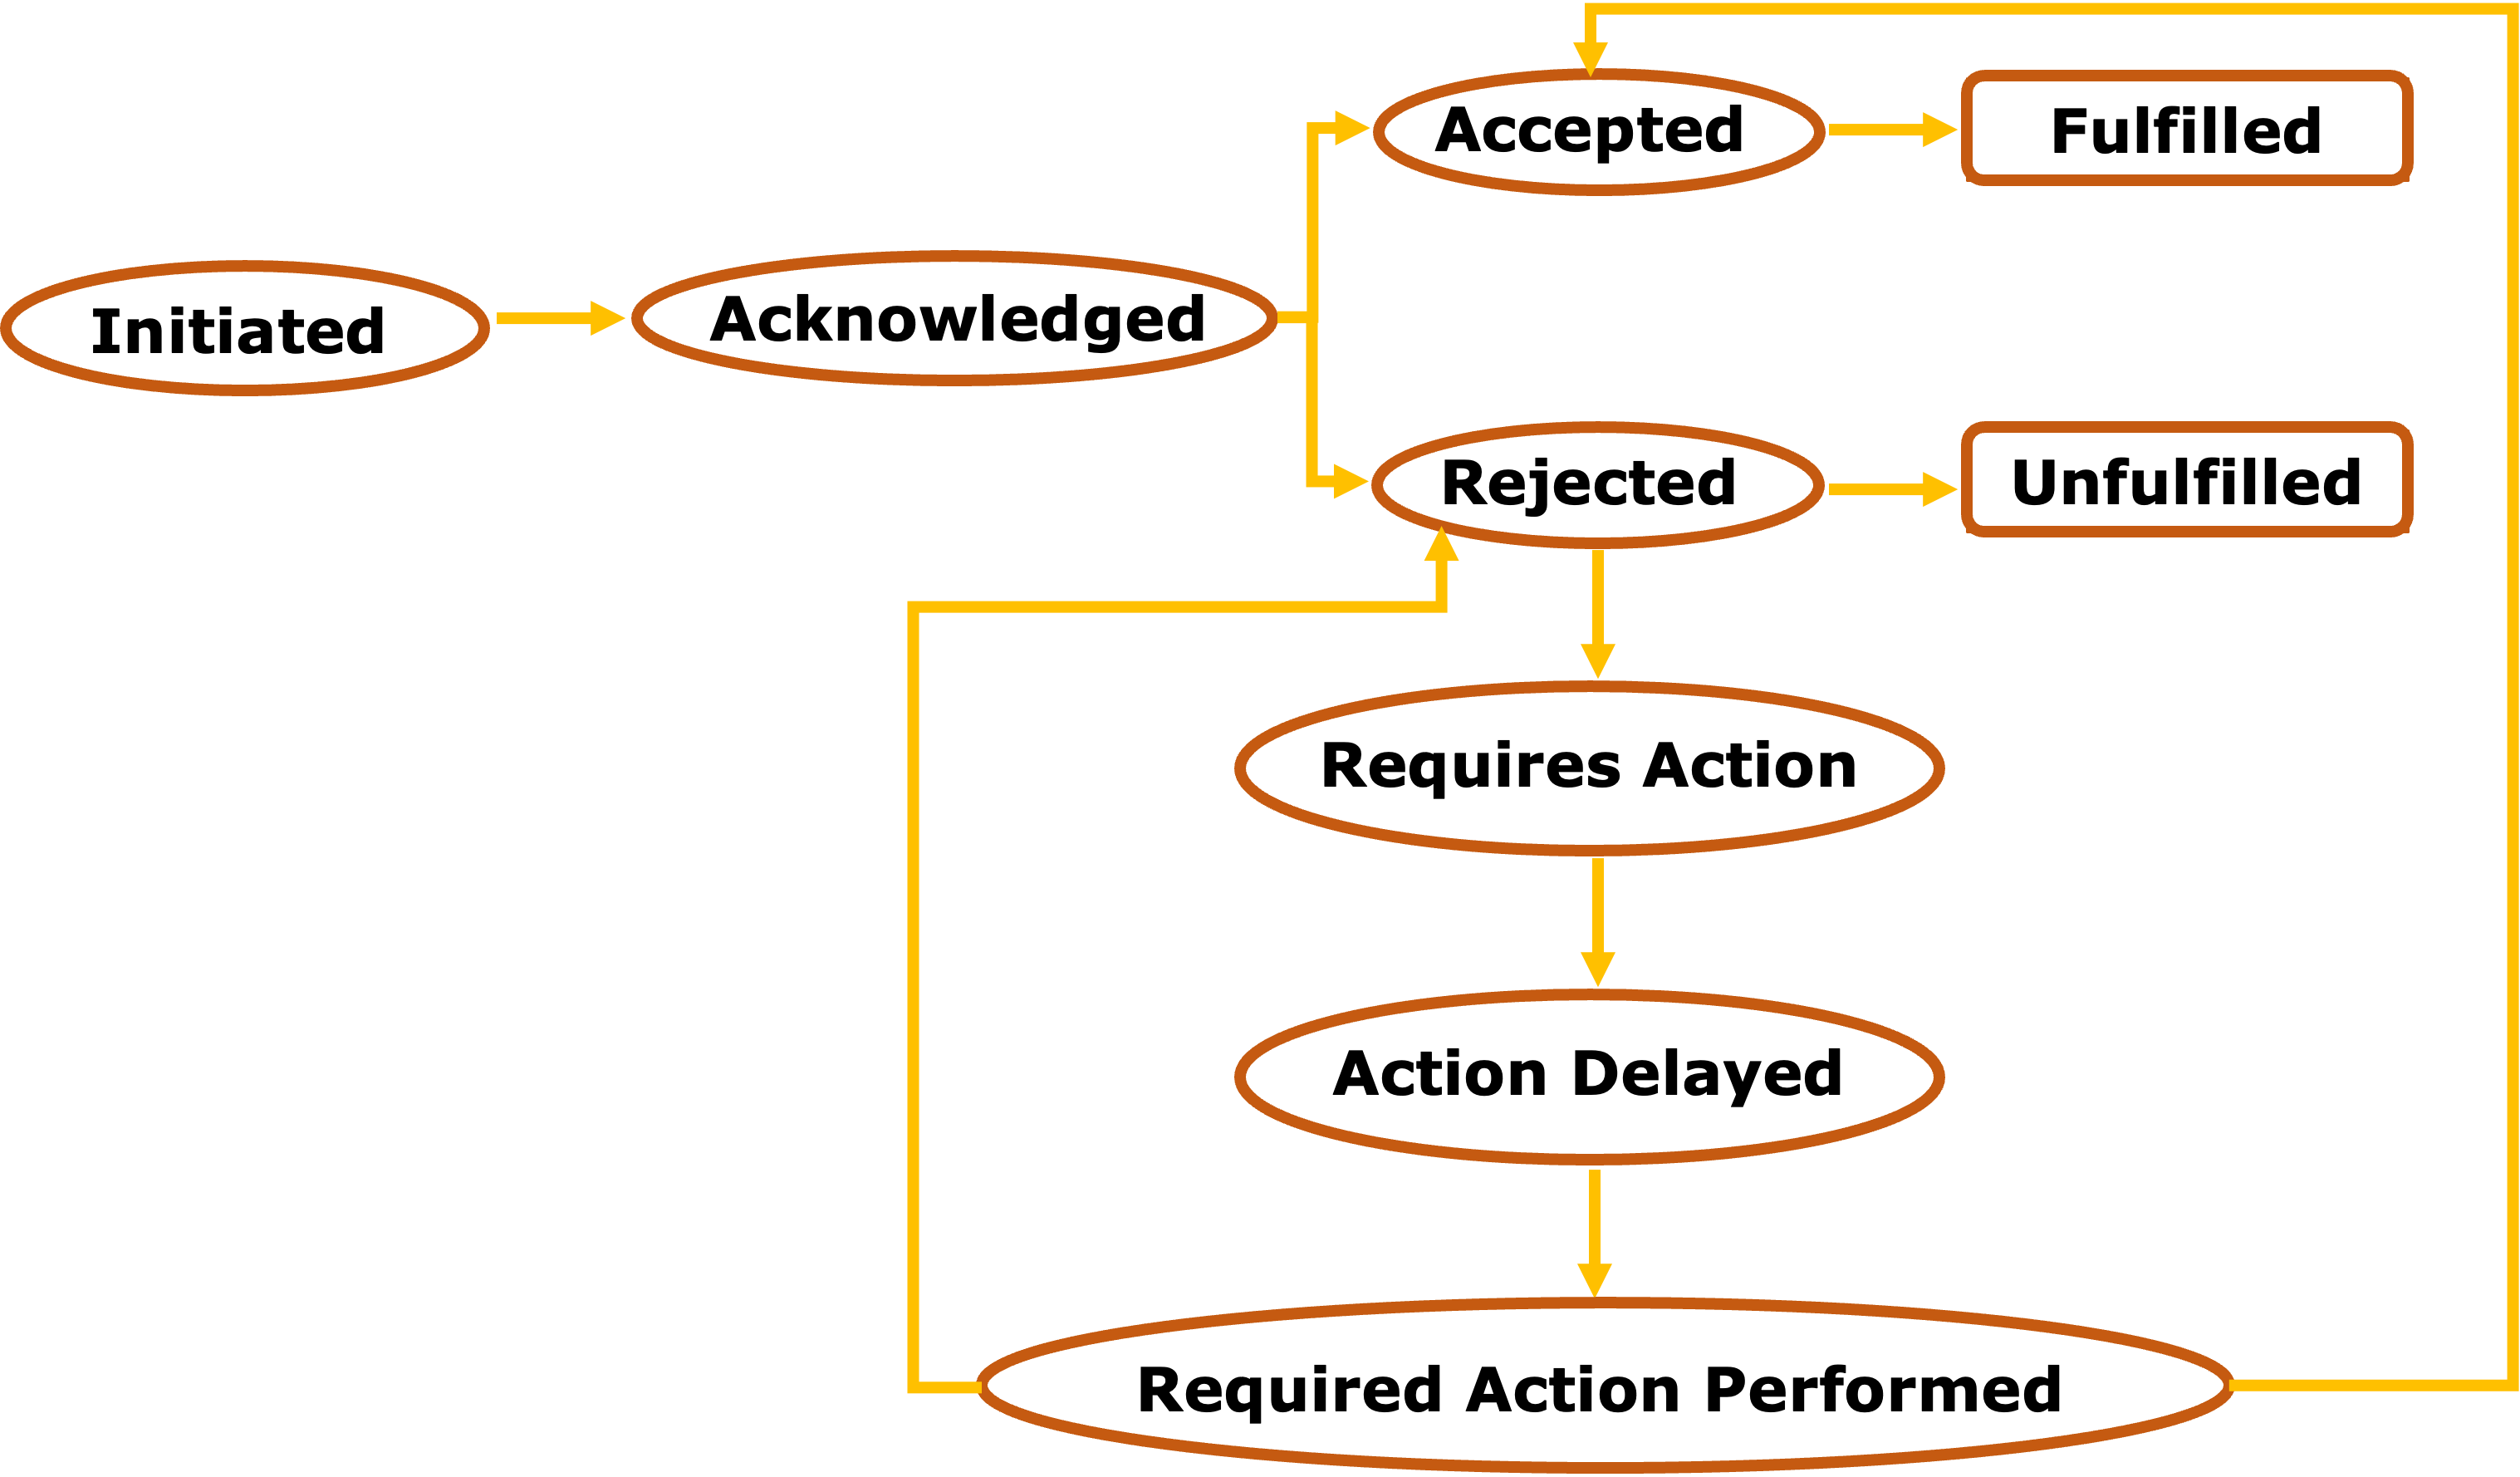
\includegraphics[width=0.7\textwidth]{img/request-status.png}
\end{figure}

Moreover, DPV concepts can be combined with the W3C's PROV-O recommendation to track the provenance of a right exercising activity instance.
This allows for the representation of provenance details, such as the entities involved in the activity, i.e., \texttt{prov:wasAssociatedWith}, or the data/notice generated by the activity, i.e., \texttt{prov:generated}. The \texttt{prov:actedOnBehalfOf} property can also be used to represent delegation or representation, for example, when a parent exercises a right on behalf of a child.
%Similar to notices, temporal information, descriptions, and identifiers of the activities, along with their creators or publishers, can be recorded using DCMI Metadata Terms.
Listing~\ref{lst:activity} provides an example of an activity where the data controller requires further action from the data subject to be able to proceed with the request. The required action is defined using a \texttt{dpv:Process}.
Examples for the whole lifecycle of activities are provided in the proposed specification.
Furthermore, the proposed model for right exercising activities is generic enough to support the representation of rights from other jurisdictions and can be easily extended if the need arises.

\begin{listing}[ht]
\caption{Right exercise activity where the data controller requires further action from the data subject to be able to proceed with the request.}
\label{lst:activity}
\begin{minted}{turtle}
ex:SARRequiresAction a dpv:RightExerciseActivity, prov:Activity ;
    dcterms:description "Data controller requires further action from data subject" ;
    dcterms:created "2023-11-02T16:09:21"^^xsd:dateTime ;
    prov:wasAssociatedWith ex:DataController ;
    dpv:hasDataSubject ex:DataSubject ;
    dpv:hasStatus dpv:RequestRequiresAction ;
    dpv:hasJustification justifications:IdentityVerificationFailure ;
    dpv:hasProcess [
        dpv:hasPersonalData pd:OfficialID ;
        dpv:hasProcessing dpv:MakeAvailable ;
        dpv:hasPurpose dpv:IdentityVerification ;
        dpv:hasRecipientDataController ex:DataController ;
        dpv:isImplementedByEntity ex:DataSubject ] .
\end{minted}
\end{listing}

\subsection{GDPR-related rights requests as machine-executable policies}
\label{sec:policies}

DPV and ODRL can also be used for data subjects to send GDPR-related right requests in a machine-interpretable format to data controllers.
Such requests can then be integrated in their rights management processes to for automated execution of responses to data subjects' requests.
For example, systems that use an ODRL evaluator based on the formal semantics of ODRL~\cite{fornara_odrl_2024} can assess policies to determine which ones are active, have been violated, or have been fulfilled, to respond consistently and interoperably to rights-related requests.
As such, GDPR's data subject rights described in Articles 15 to 22 can be instantiated as ODRL policies containing permissions, prohibitions and obligations to data controllers to act upon or fulfil.
Generic policies for each right are available in the proposed specification.
Listing~\ref{lst:policy} provides an example of a request to exercise GDPR's right to erasure.
It can be represented as an obligation to delete a data subject's personal data based on one of the grounds specified in Article 17.1.
These grounds can be detailed using DPV's justifications, e.g., the data is no longer necessary in relation to the purposes for which it was processed~--\texttt{justifications:NonNecessityObjection}.
Additionally, Article 19 requires that if the data has been shared with recipients, the data controller must inform the data subject about these recipients.

\begin{listing}[ht]
\caption{Request policy to exercise GDPR right to erasure.}
\label{lst:policy}
\begin{minted}{turtle}
ex:delete-request a odrl:Request ;
    odrl:uid "3456-7890-1234-5678-9012"^^xsd:string ;
    dcterms:description "Data subject requests data controller to delete their data." ;
    odrl:obligation ex:DS-delete-data ;
    odrl:obligation ex:DS-delete-notice .

ex:DS-delete-data a odrl:Duty ;
    dpv:hasRight eu-gdpr:A17 ;
    odrl:target ex:DS-data ;
    odrl:assigner ex:DataSubject ;
    odrl:assignee ex:DataController ;
    odrl:action odrl:delete ;
    odrl:constraint ex:DS-delete-justification .

ex:DS-delete-justification a odrl:Constraint ;
    odrl:leftOperand dpv:Justification ;
    odrl:operator odrl:eq ;
    odrl:rightOperand justifications:NonNecessityObjection .

ex:DS-delete-notice a odrl:Duty ;
    dpv:hasRight eu-gdpr:A19 ;
    odrl:action odrl:inform ;
    odrl:informedParty ex:DataSubject ;
    odrl:informingParty ex:DataController ;
    odrl:target ex:DS-RightsRecipientsNotice .

ex:DS-RightsRecipientsNotice a eu-gdpr:RightsRecipientsNotice .
\end{minted}
\end{listing}

\section{Conclusions and Future Work}
\label{sec:conclusions}

In this article, we proposed a semantic specification for representing information about rights exercisement and management based on the requirements of the GDPR.
The specification provides a machine-interpretable and executable model to represent information regarding data subject rights, concepts to justify their fulfilment or non-fulfilment, notices to communicate about them with other entities, records for auditing and policies for automated execution of responses to rights requests.
Through these, we hope to enable related tools and processes to handle obligations related to rights in an interoperable manner. 

\bibliography{ref}
\bibliographystyle{vancouver}

\end{document}
